\documentclass{beamer}
\usepackage[english,russian]{babel}
\usepackage[utf8x]{inputenc}
\usepackage{listings}
\lstset{basicstyle=\footnotesize}
% Стиль презентации
\usetheme{Warsaw}
\graphicspath{{images/}}
\begin{document}
	\title[XLVI Конференция Университета ИТМО]{Информационно-поисковая система\\ научного и образовательного контента\\ на основе открытых данных}  
	\author[Герасин О.В.]{Герасин Олег}
	\logo{
\includegraphics[width=2cm,height=2cm,keepaspectratio]{itmo.png}}
	\institute{Студент группы P4117}
	\date{Санкт-Петербург, 2017} 
	% Создание заглавной страницы
	\frame{\titlepage} 
	% Автоматическая генерация содержания
	%\frame{\frametitle{Содержание}\tableofcontents} 
	\begin{frame}{Введение}
		%\pause
		%\begin{block}{Сетевая технология}
		%Сетевая технология	- это согласованный набор стандартных протоколов и реализующих их программно-аппаратных средств, достаточный для построения локальной вычислительной сети.
		%\end{block}
	\end{frame}

	\begin{frame}{Аналоги}
%		\pause
%		\begin{block}{Изобретение}
%			Ethernet был изобретён 22 мая 1973 года.
%		\end{block}
%		\pause
%		\begin{block}{Продвижение}
%			В сентябре 1982 года был представлен первый сетевой адаптер для ПК. 
%		\end{block}
%		\pause
%		\begin{block}{Коммутаторы}
%			С 1992 года в мире активно применяются коммутаторы (switch).
%		\end{block}		
		
	\end{frame}	
	
	\begin{frame}{Описание подхода}
%		\pause
		 \begin{center}
		 	\includegraphics[scale=0.5]{uml.png}  
		 \end{center}
	\end{frame}	
	
	\begin{frame}{Прототип}
	%	\pause
		 \begin{center}
		 	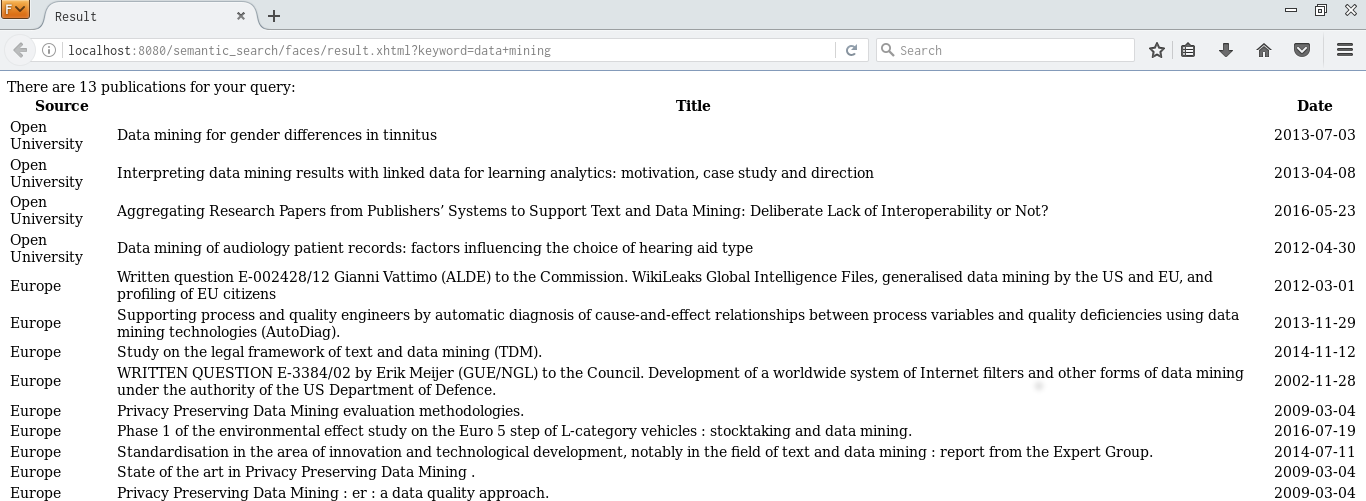
\includegraphics[scale=0.23]{results.png}  
		 \end{center}
	\end{frame}	
	\begin{frame}{Пример запроса}
		%\pause
		\begin{center}
		 \lstinputlisting{sparql.txt}
		\end{center}
	\end{frame}
	
	\begin{frame}{Перспективы}
%		\pause
%		\begin{columns}
%			\column{.5\textwidth}
%			\begin{center}
%			\includegraphics[scale=0.07]{eth.jpg}\\
%			\pause
%			\includegraphics[scale=0.5]{opt.jpg}
%						\pause
%			\end{center}
%			\column{.5\textwidth}
%			\begin{center}			
%			\includegraphics[scale=0.4]{sw}\\
%			\pause
%			\includegraphics[scale=0.3]{par.jpg}
%			\end{center}
%		\end{columns}
	\end{frame}
	
	\begin{frame}
		\frametitle{Заключение}
%		\pause
%		Достоинства
%		\begin{itemize}
%			\item<3-> Дешевизна
%			\item<4-> Большой опыт использования
%			\item<5-> Продолжающиеся нововведения
%			\item<6-> Богатство выбора оборудования
%		\end{itemize}
	\end{frame}	
	
	\begin{frame}{Список использованных источников}
		%\pause
%		\begin{thebibliography}{10}
%			\beamertemplatebookbibitems
%			\bibitem{Wiki}
%			{\sc https://ru.wikipedia.org/}, {\em Свободная энциклопедия [Электронный ресурс]}.
%			\bibitem{sernam}
%			{\sc http://sernam.ru/}, {\em Научная библиотека [Электронный ресурс]}.
%		\end{thebibliography}
	\end{frame}
\end{document}